\chapter{Функции обработчика прерывания системного таймера}

\section{Unix/Linux}

\textbf{По тику}
\begin{itemize}
	\item Инкремент счётчика реального времени и других счётчиков времени(например в SVR4, lbolt -- счётчик тиков с момента запуска системы);
	\item Декремент кванта текущего потока;
	\item Инкремент счётчиков процессорного времени в режимах задачи и ядра;
	\item Декремент счётчика тиков отложенных вызовов. Если счётчик обнулился, то установка флага запуска ожидающего вызова.
\end{itemize}

\textbf{По главному тику}
\begin{itemize}
	\item Пробуждение системных процессов ( например pagedaemon, swapper для Unix, kswapd для Linux);
	\item Отложенный вызов функций планировщика (пересчёт приоритетов);
	\item Декремент счётчиков времени, до посылки сигналов будильников SIGVTALRM, SIGPROF, SIGALRM.
\end{itemize}

\textbf{По кванту}
\begin{itemize}
	\item Посылка сигнала SIGXCPU о том, что процесс израсходовал квант.
\end{itemize}

\section{Windows}

\textbf{По тику}
\begin{itemize}
	\item Инкремент счётчика реального времени;
	\item Декремент кванта текущего потока;
	\item Декремент счётчика тиков отложенных вызовов;
	\item Запись адреса выполняемого кода при активном профилировании ядра.
\end{itemize}

\textbf{По главному тику}
\begin{itemize}
	\item Запуск диспетчеризации настройки баланса(каждую секунду);
\end{itemize}

\textbf{По кванту}
\begin{itemize}
	\item Отложенный вызов (DPC) диспетчеризации потоков.
\end{itemize}


\chapter{Пересчёт динамических приоритетов}

Операционные системы Unix и Windows являются системами разделения времени с динамическим приоритетами, соответственно процессорное время выделяется процессам в соответствии с их приоритетом, при этом их приоритеты меняются по ходу выполнения программы.

\section{Unix/Linux}

Планировщик Unix предоставляет процессор каждому процессу на небольшой промежуток времени, который называется \textbf{квантом времени}, а затем переключает на следующий процесс. При переключении процессов планировщик заставляет процессор выполнить \textbf{переключение контекста}. При этом действии ядро системы сохраняет аппаратный контекст, то есть текущие значения регистров общего назначения, управления памятью и других. После сохранения, ядро системы загружает аппаратный контекст процесса, который будет выполняться.

В системах Unix планировщик выбирает обладающие наиболее высоким приоритетом, среди всех. При этом если процессы обладают одинаковым приоритетом, то применяется вытесняющее квантование времени для этих процессов. При этом изменение приоритетов происходит динамически и если какой-то из высокоприоритетных процессов станет готов к выполнению, то он вытеснит текущий процесс, даже если тот не израсходовал свой квант времени.


Традиционное ядро Unix является строго невытесняющим (или по-другому <<непрерываемым>>), то есть процесс находящийся в режиме ядра не может быть вытеснен другим, даже более высокоприоритетным процессом. Выполняющийся процесс может добровольно освободить процессор, в случае блокирования на ресурсе, или вытеснен при переходе в режим задачи. Такой подход решает проблемы синхронизации, связанные с одновременным доступом нескольких процессов к одним и тем же объектам ядра.

Современные системы Unix/Linux являются вытесняющими, то есть процесс в режиме ядра может быть вытеснен более высокоприоритетным процессом.

Приоритет процесса может представляться любым целым числом в диапазоне от 0 до 127. Для системы  4.3BSD UNIX чем ниже это число, тем более высокий приоритет имеет процесс. Значения от 0 до 49 зарезервированы для режима ядра, остальные 50-127 отведены под прикладные процессы.

Структура $proc$, описывающая дескриптор процесса содержит следующие поля, характеризующие приоритет процесса:

\begin{itemize}
	\item $p\_pri$ -- Текущий приоритет планирования;
	\item $p\_usrpri$ -- Приоритет процесса в режиме задачи;
	\item $p\_cpu$ -- Результат последнего измерения использования процессора;
	\item $p\_nice$ -- Фактор <<Любезности>> процесса, устанавливаемый пользователем.
\end{itemize}

Поле $p\_pri$ используется планировщиком для принятия решения о том, какой процесс направить на выполнение. Значение $p\_pri$ совпадает с $p\_usrpri$, когда процесс находится в режиме задачи. Когда процесс просыпается после блокирования в системном вызове, его значение $p\_pri$ понижается, то есть приоритет повышается, для того, чтобы дать ему предпочтение среди остальных процессов.


Ядро системы связывает приоритет сна с событием или ожидаемым ресурсом. Когда блокированный процесс просыпается ядро устанавливает его значение $p\_pri$ равным приоритету сна или ресурса, при этом все эти приоритеты лежат в диапазоне 0-49, что повышает приоритет процесса по сравнению с процессами в режиме задачи. На рисунке~\ref{fig:sleep} приведены значения приоритетов сна для систем 4.3BSD UNIX и SCO
UNIX (OpenServer 5.0).

\begin{figure}[H]
	\centering
	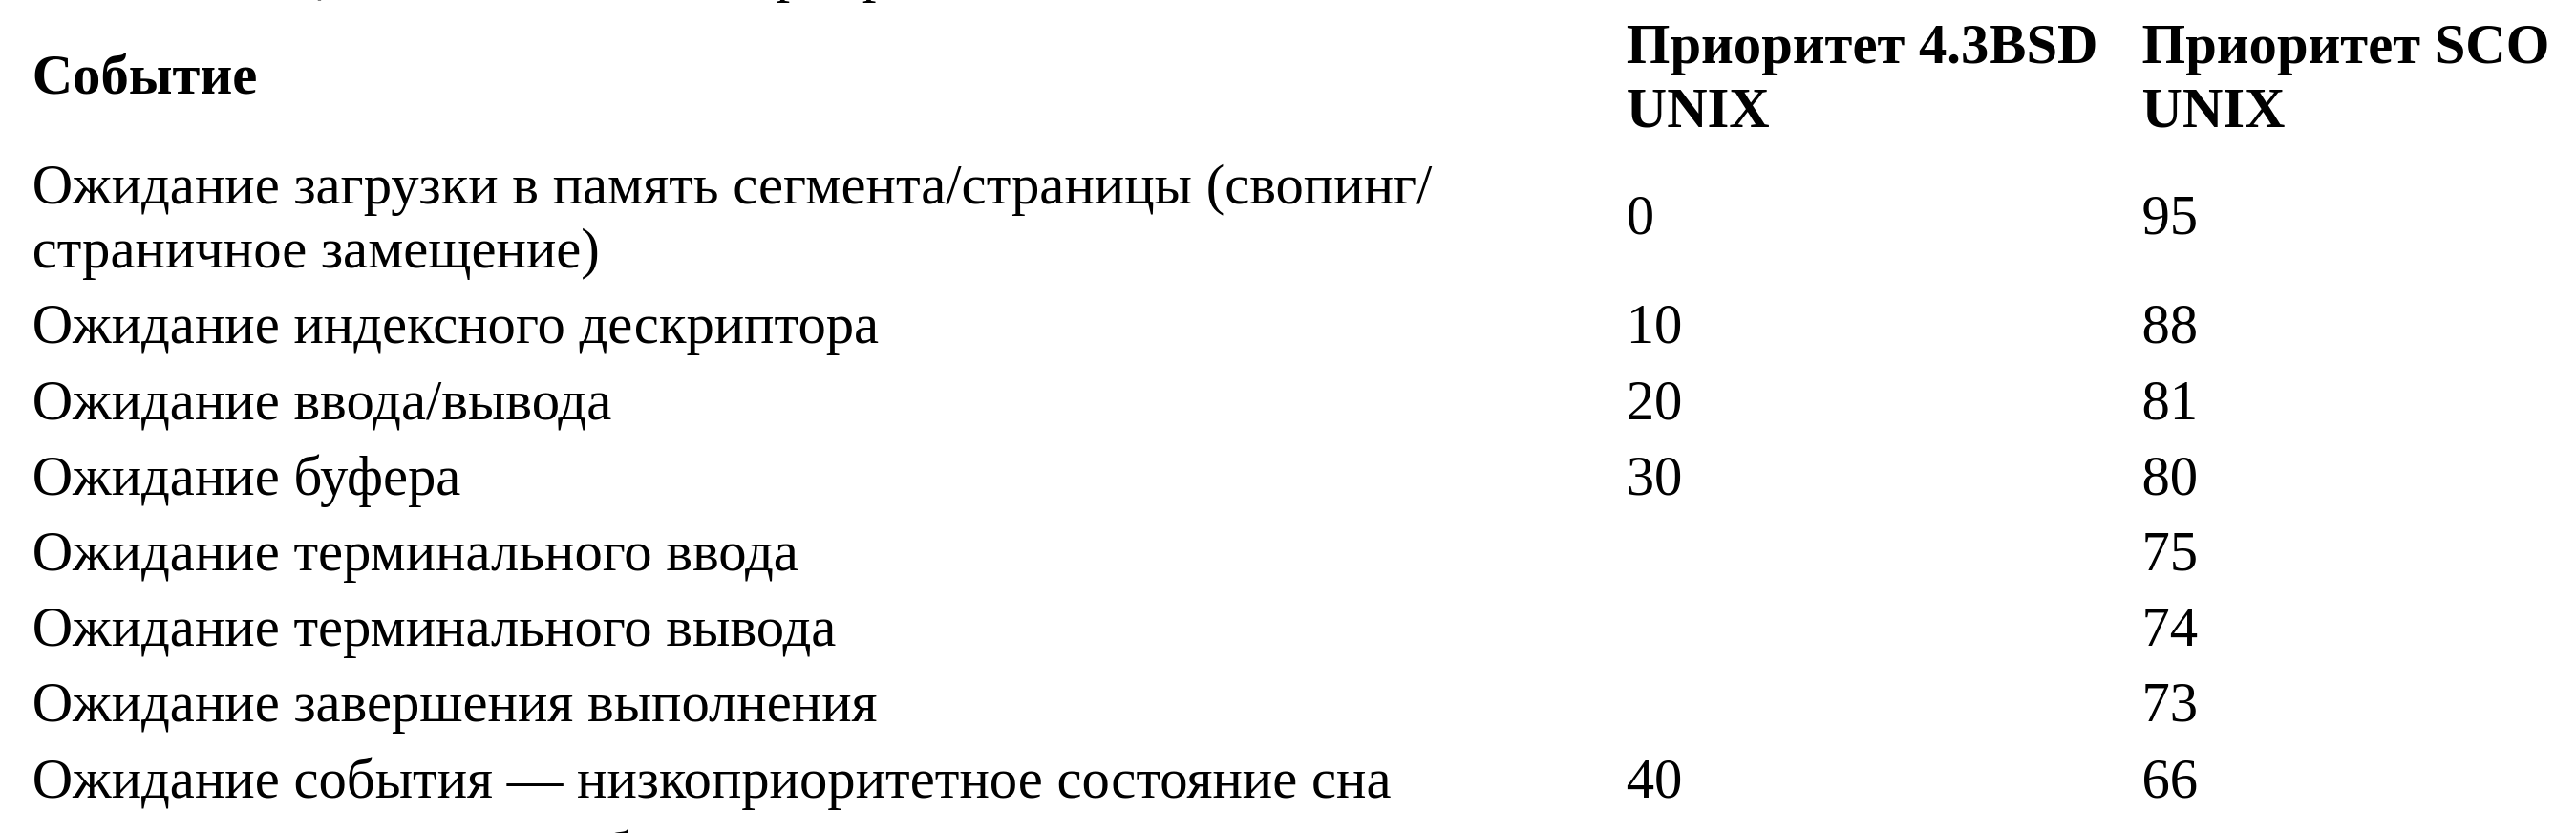
\includegraphics[width=0.9\textwidth]{sleep}
	\caption{Системные приоритеты сна}
	\label{fig:sleep}
\end{figure}

После завершения системного вызова перед возвращением в режим задачи ядро восстанавливает приоритет режима задачи, сохранённый перед выполнением системного вызова. Это может привести к понижению приоритета, что, в свою очередь, вызовет переключение контекста.

В режиме задачи приоритет зависит от двух факторов: <<любезности>> и последней измеренной величиной использования процессора.

Степень <<любезности>> процесса определяется числом от 0 до 39 со значением 20 по умолчанию. Увеличение этого числа приводит к уменьшению приоритета процесса, таким образом такой процесс будет уступать места более высокоприоритетным процессам. Уменьшить эту величину может только суперпользователь, так как это приведёт к увеличению приоритета процесса.

Поле $p_cpu$ содержит последний результат измерения использования процессора. Эта величина увеличивается на 1 на каждом тике, при выполнении процесса, вплоть до максимального значения в 127. Также каждую секунду ядро выпускает процедуру $schedcpu()$ которая уменьшает значение $p_cpu$ по фактору <<полураспада>>. В 4.3BSD Unix для этого используется формула~\ref{eq:factor}

\begin{equation}
	\label{eq:factor}
	p\_cpu = p\_cpu\frac{2*load\_average}{2*load\_average+1},
\end{equation}
где $load\_average$ -- среднее количество готовых к выполнению процессов за последнюю секунду. После расчёта $p\_cpu$ рассчитывается приоритет процесса в режиме задачи~\ref{eq:prior-unix}.

\begin{equation}
	\label{eq:prior-unix}
	p\_usrpri = PUSER + \frac{p\_cpu}{4} + 2*p\_nice,
\end{equation}
где $PUSER = 50$ -- базовый приоритет процессов в пользовательском режиме.

В результате долгое использование процессора повышает $p\_cpu$, что понижает приоритет процесса, с другой стороны долгое нахождение в очереди процессов повышает его приоритет за счёт фактора <<полураспада>>. Такая схема предотвращает бесконечное откладывание.

\section{Windows}

Планировщик Windows реализует приоритетная, вытесняющая система планирования. Единицей диспетчеризации, как и в случае unix, является процесс, которому при его создании задаётся базовый приоритет. Приоритеты потоков задаются относительно приоритета процесса. 

Как и в случае планировщика Unix, планировщик Windows предоставляет потоку квант времени, при этом для выполнения всегда выбирается готовый к запуску поток с наивысшим приоритетом.
Поток может перестать выполняться, если:

\begin{itemize}
	\item появился более высокоприоритетный поток (например вышел из ожидания). Тогда текущий поток будет вытеснен более высокоприоритетным потоком;
	\item поток добровольно отказался от кванта, путём входа в ожидание какого-нибудь объекта (события, мьютекса, семафора, т.д.);
	\item квант, выделенный потоку закончился. Тогда квант может быть передан более высокоприоритетным потокам, если они есть, потокам с тем же приоритетам по очереди, если они есть, либо тому же самому потоку, если есть только потоки с более низким приоритетом.
\end{itemize}

Приоритет в Windows задаётся одним из 32 значений в диапазоне от 0 до 31, при этом 0 зарезервирован для потока обнуления страниц, 1-15 -- изменяющиеся уровни, а 16-31 -- уровни реального времени. 

\begin{figure}[H]
	\centering
	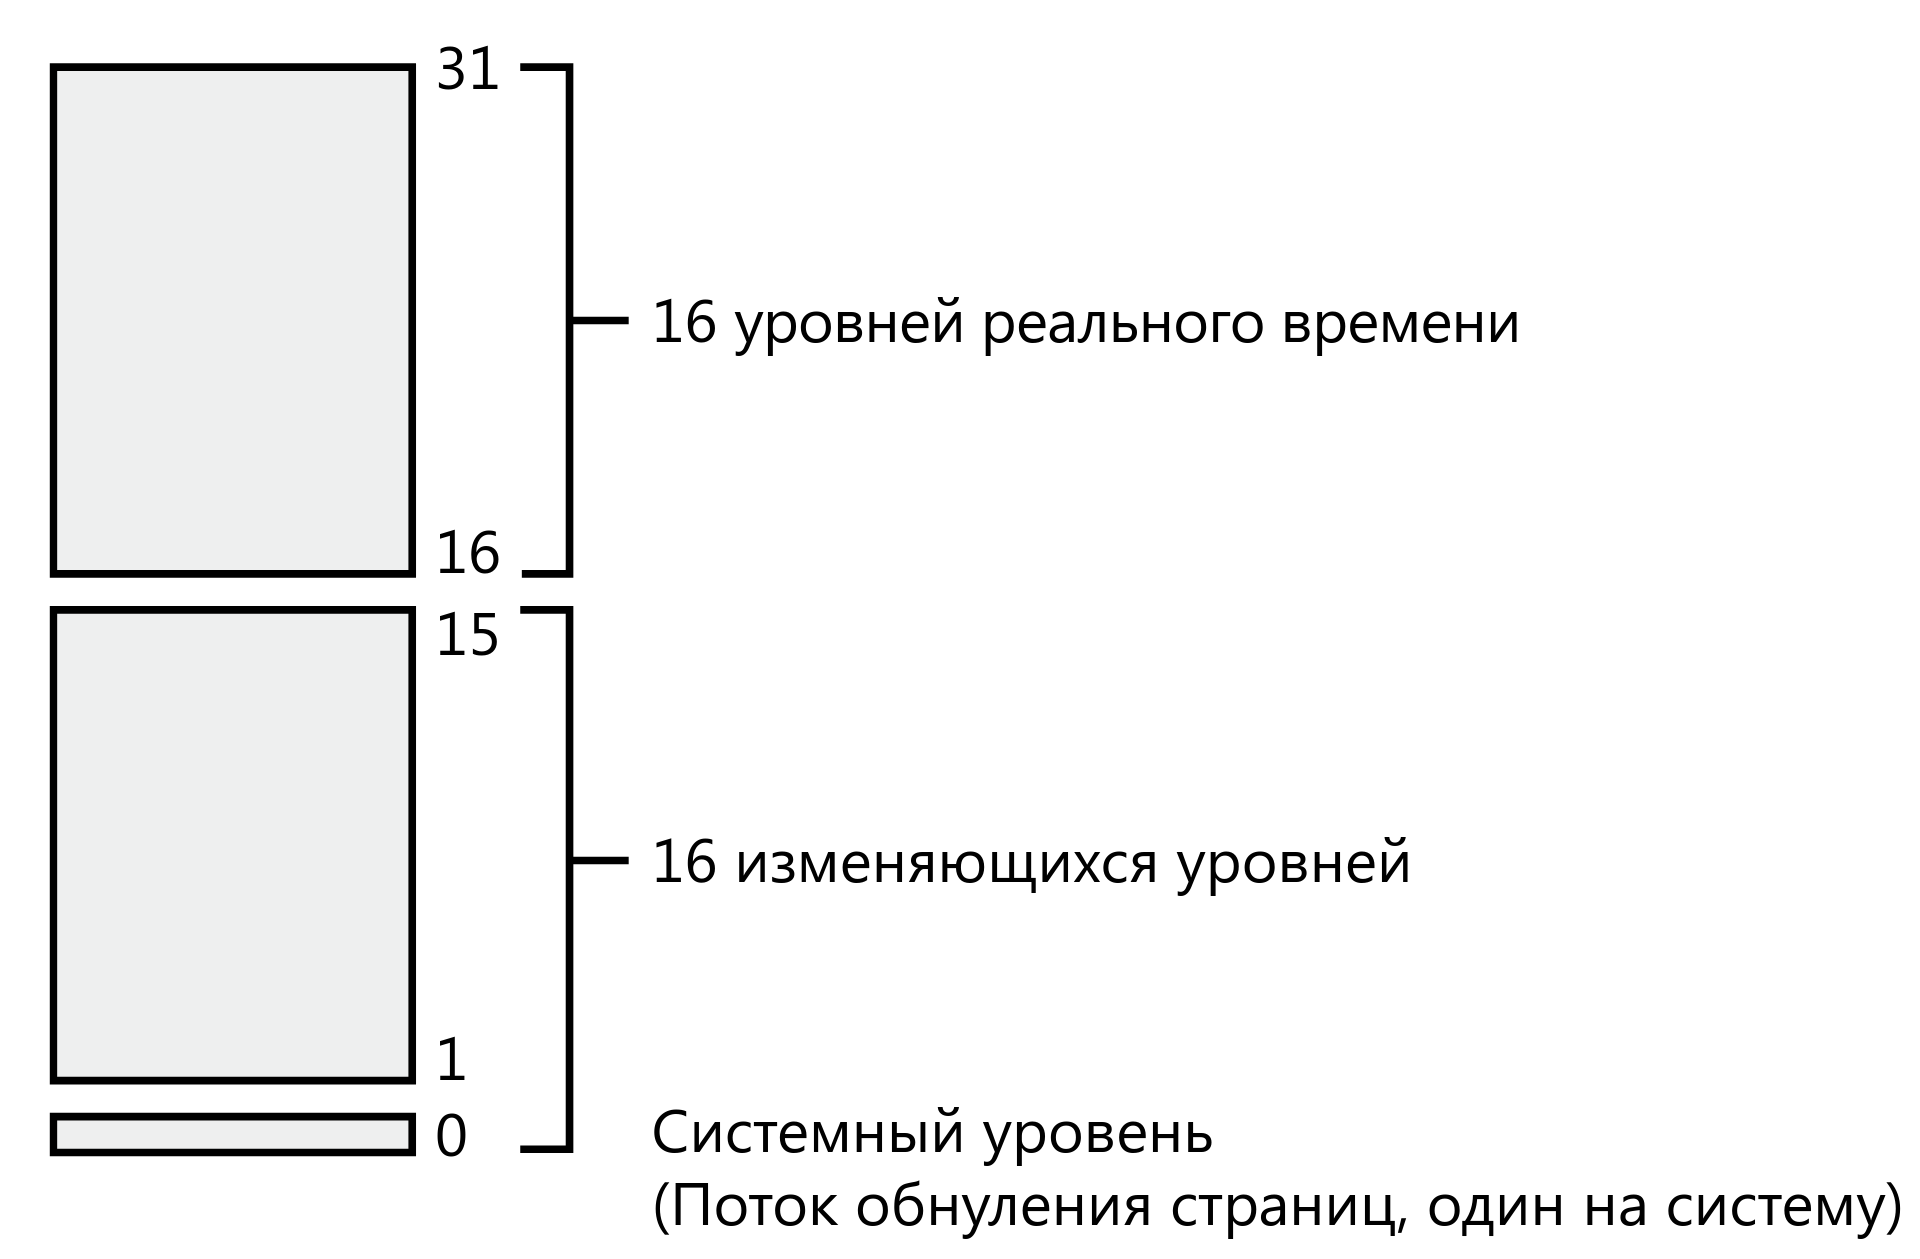
\includegraphics[width=0.6\textwidth]{levels}
	\caption{Уровни приоритета потоков}
	\label{fig:levels}
\end{figure}

Приоритет процесса присваивается Windows API при создании процесса и может быть одним из 6 значений:
\begin{itemize}
	\item Реального времени -- Real-time (4); 
	\item Высокий -- High (3);
	\item Выше обычного -- Above Normal (7);
	\item Обычный -- Normal (2);
	\item Ниже обычного -- Below Normal (5);
	\item Простоя -- Idle (1).
\end{itemize}

Затем для отдельных потоков назначается относительный приоритет потока, который имеет либо положительное значение либо отрицательное:

\begin{itemize}
	\item Критичный по времени -- Time-critical (15);
	\item Наивысший -- Highest (2);
	\item Выше обычного -- Above-normal (1);
	\item Обычный -- Normal (0);
	\item Ниже обычного -- Below-normal (-1);
	\item Низший -- Lowest (-2);
	\item Простоя -- Idle (–15).
\end{itemize}

Таким образом в Windows API каждый поток имеет базовый приоритет, являющийся функцией класса приоритета процесса и его относительного приоритета процесса. На рисунке~\ref{fig:prior-win} представлена таблица, отображающая относительный приоритет и приоритет процесса на  базовый приоритет потока.

\begin{figure}[H]
	\centering
	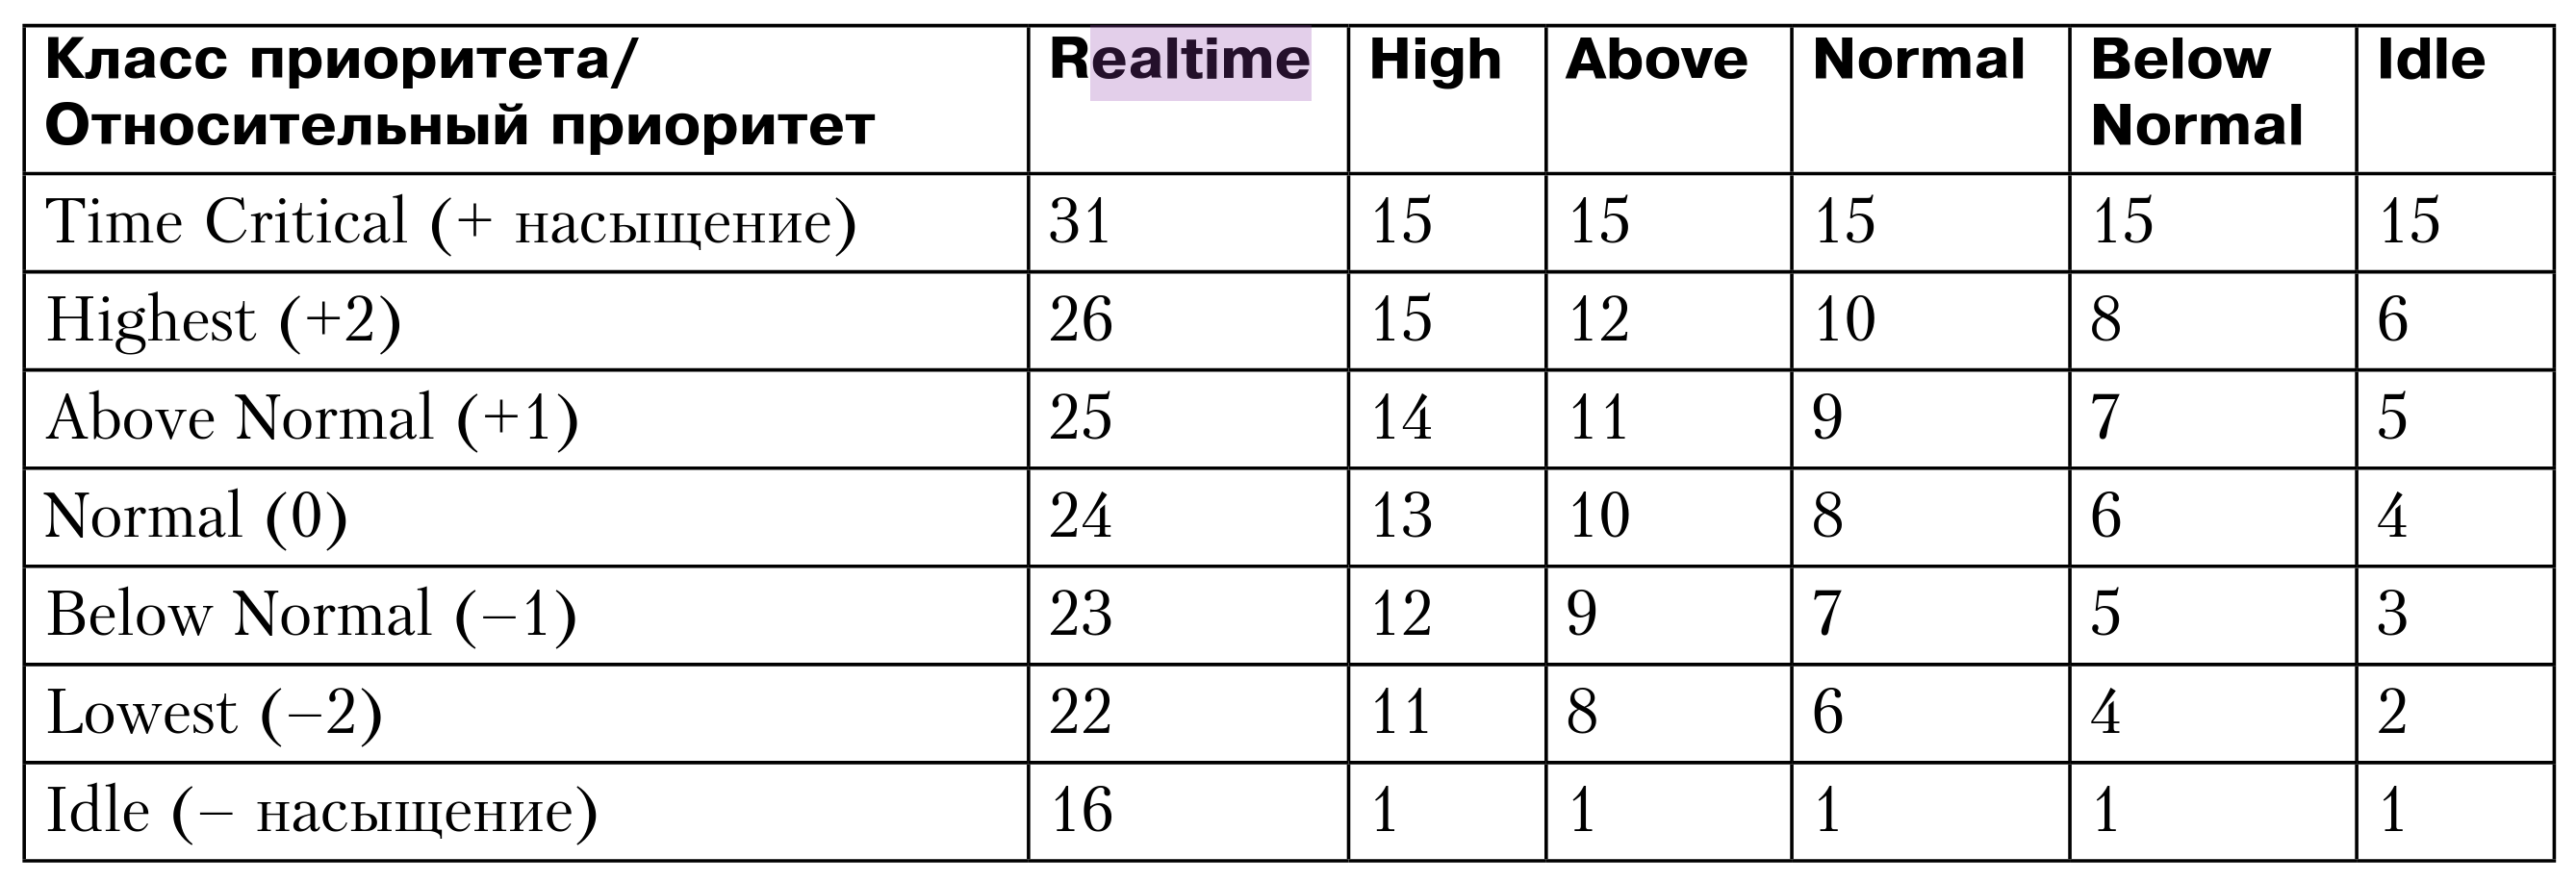
\includegraphics[width=0.9\textwidth]{prior}
	\caption{Отображение приоритетов ядра Windows на Windows API}
	\label{fig:prior-win}
\end{figure}

У каждого потока есть 2 вида приоритетов: текущий и базовый. Текущий используется планировщиком при выборе следующего потока. В общем случае текущий приоритет равен базовому, однако он может быть повышен планировщиком. Такие повышения могут иметь следующую природу:

\begin{itemize}
	\item \textbf{Повышение вследствие событий планировщика или диспетчера:} событие установлено или отправило сигнал, мьютекс был освобожден или ликвидирован, был освобожден семафор, в очередь была вставлена запись или очередь была очищена и др. -- повышение приоритета на 2;
	\item \textbf{Повышения приоритета, связанные с завершением ожидания:} увеличение приоритета потока, вышедшего из ожидания в состояние ready -- повышение приоритета на 1;
	\item \textbf{Повышение при ожидании ресурсов исполняющей системы:} если некоторый поток блокируется при получения ресурса системы, который уже находится в исключительном владении другого поток, то для избежания зависания приоритет владеющего потока повышается через некоторое время, после начала ожидания -- приоритет повышается до 14 (если был < 14);
	\item \textbf{Повышение приоритета потоков первого плана после ожидания:} большее повышение приоритета интерактивных процессов для улучшения их отзывчивости -- приоритет повышается на текущее значение переменной $PsPrioritySeparation$;
	\item \textbf{Повышения приоритета, связанные с перезагруженностью
	центрального процессора:} раз в секунду диспетчер настройки баланса, который является частью системного потока, канирует очередь готовых потоков в поиске тех из них, которые находятся в состоянии ready около 4 секунд и повышает их приоритет -- приоритет повышается до 15 (если был < 15);
	\item \textbf{Повышение приоритета после завершения ввода-вывода:} Windows дает временное повышение приоритета при завершении определенных операций ввода-вывода, при этом потоки, ожидавшие ввода-вывода, имеют	больше шансов сразу же запуститься и обработать то, чего они ожидали. Рекомендованные значения для данных повышений представлены на рисунке~\ref{fig:inout}, хотя действительные значения повышения определяются драйвером соответствующего устройства (как видно из рисунка аудио устройство имеет более высокий приоритет из-за того, что слух человека чувствительней к задержкам, по сравнению со зрением).
	\begin{figure}[H]
		\centering
		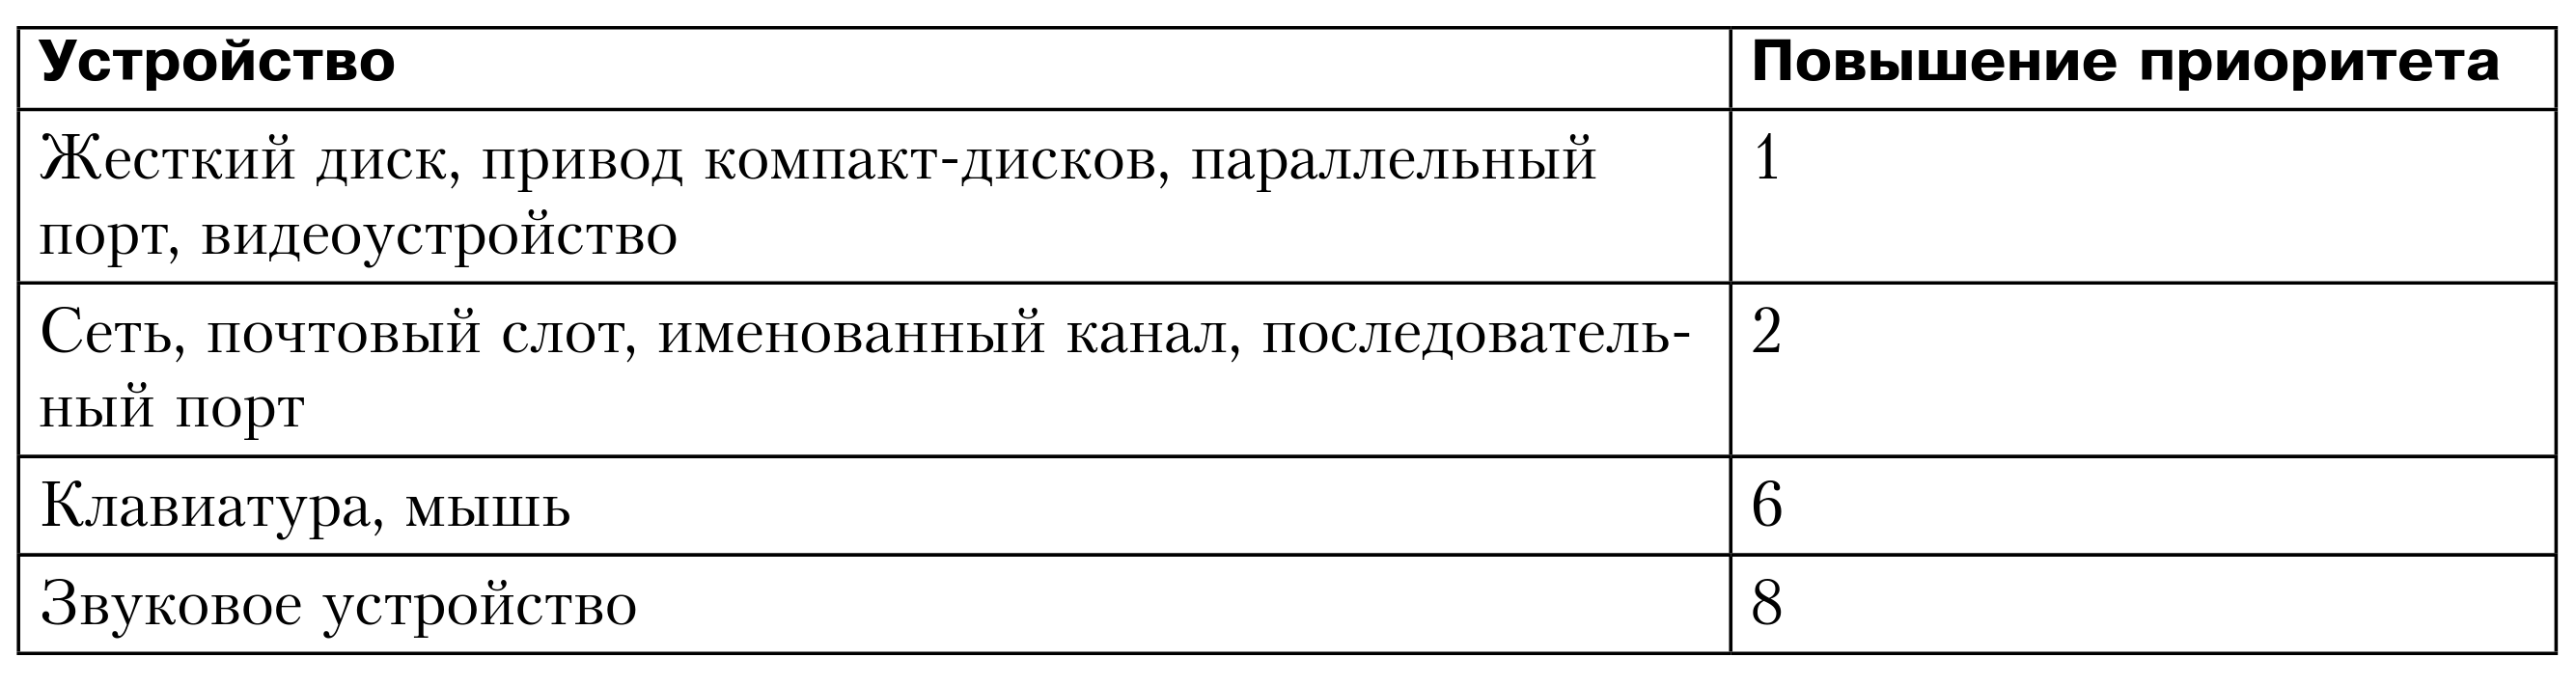
\includegraphics[width=0.9\textwidth]{inout}
		\caption{Рекомендуемые значения повышения приоритета}
		\label{fig:inout}
	\end{figure}
\end{itemize}

Большинство описанных выше повышений приоритетов перестают действовать после завершения кванта или нескольких, выделенных процессу. На рисунке~\ref{fig:priorgraph} представлен пример повышения и понижения приоритетов.

\begin{figure}[H]
	\centering
	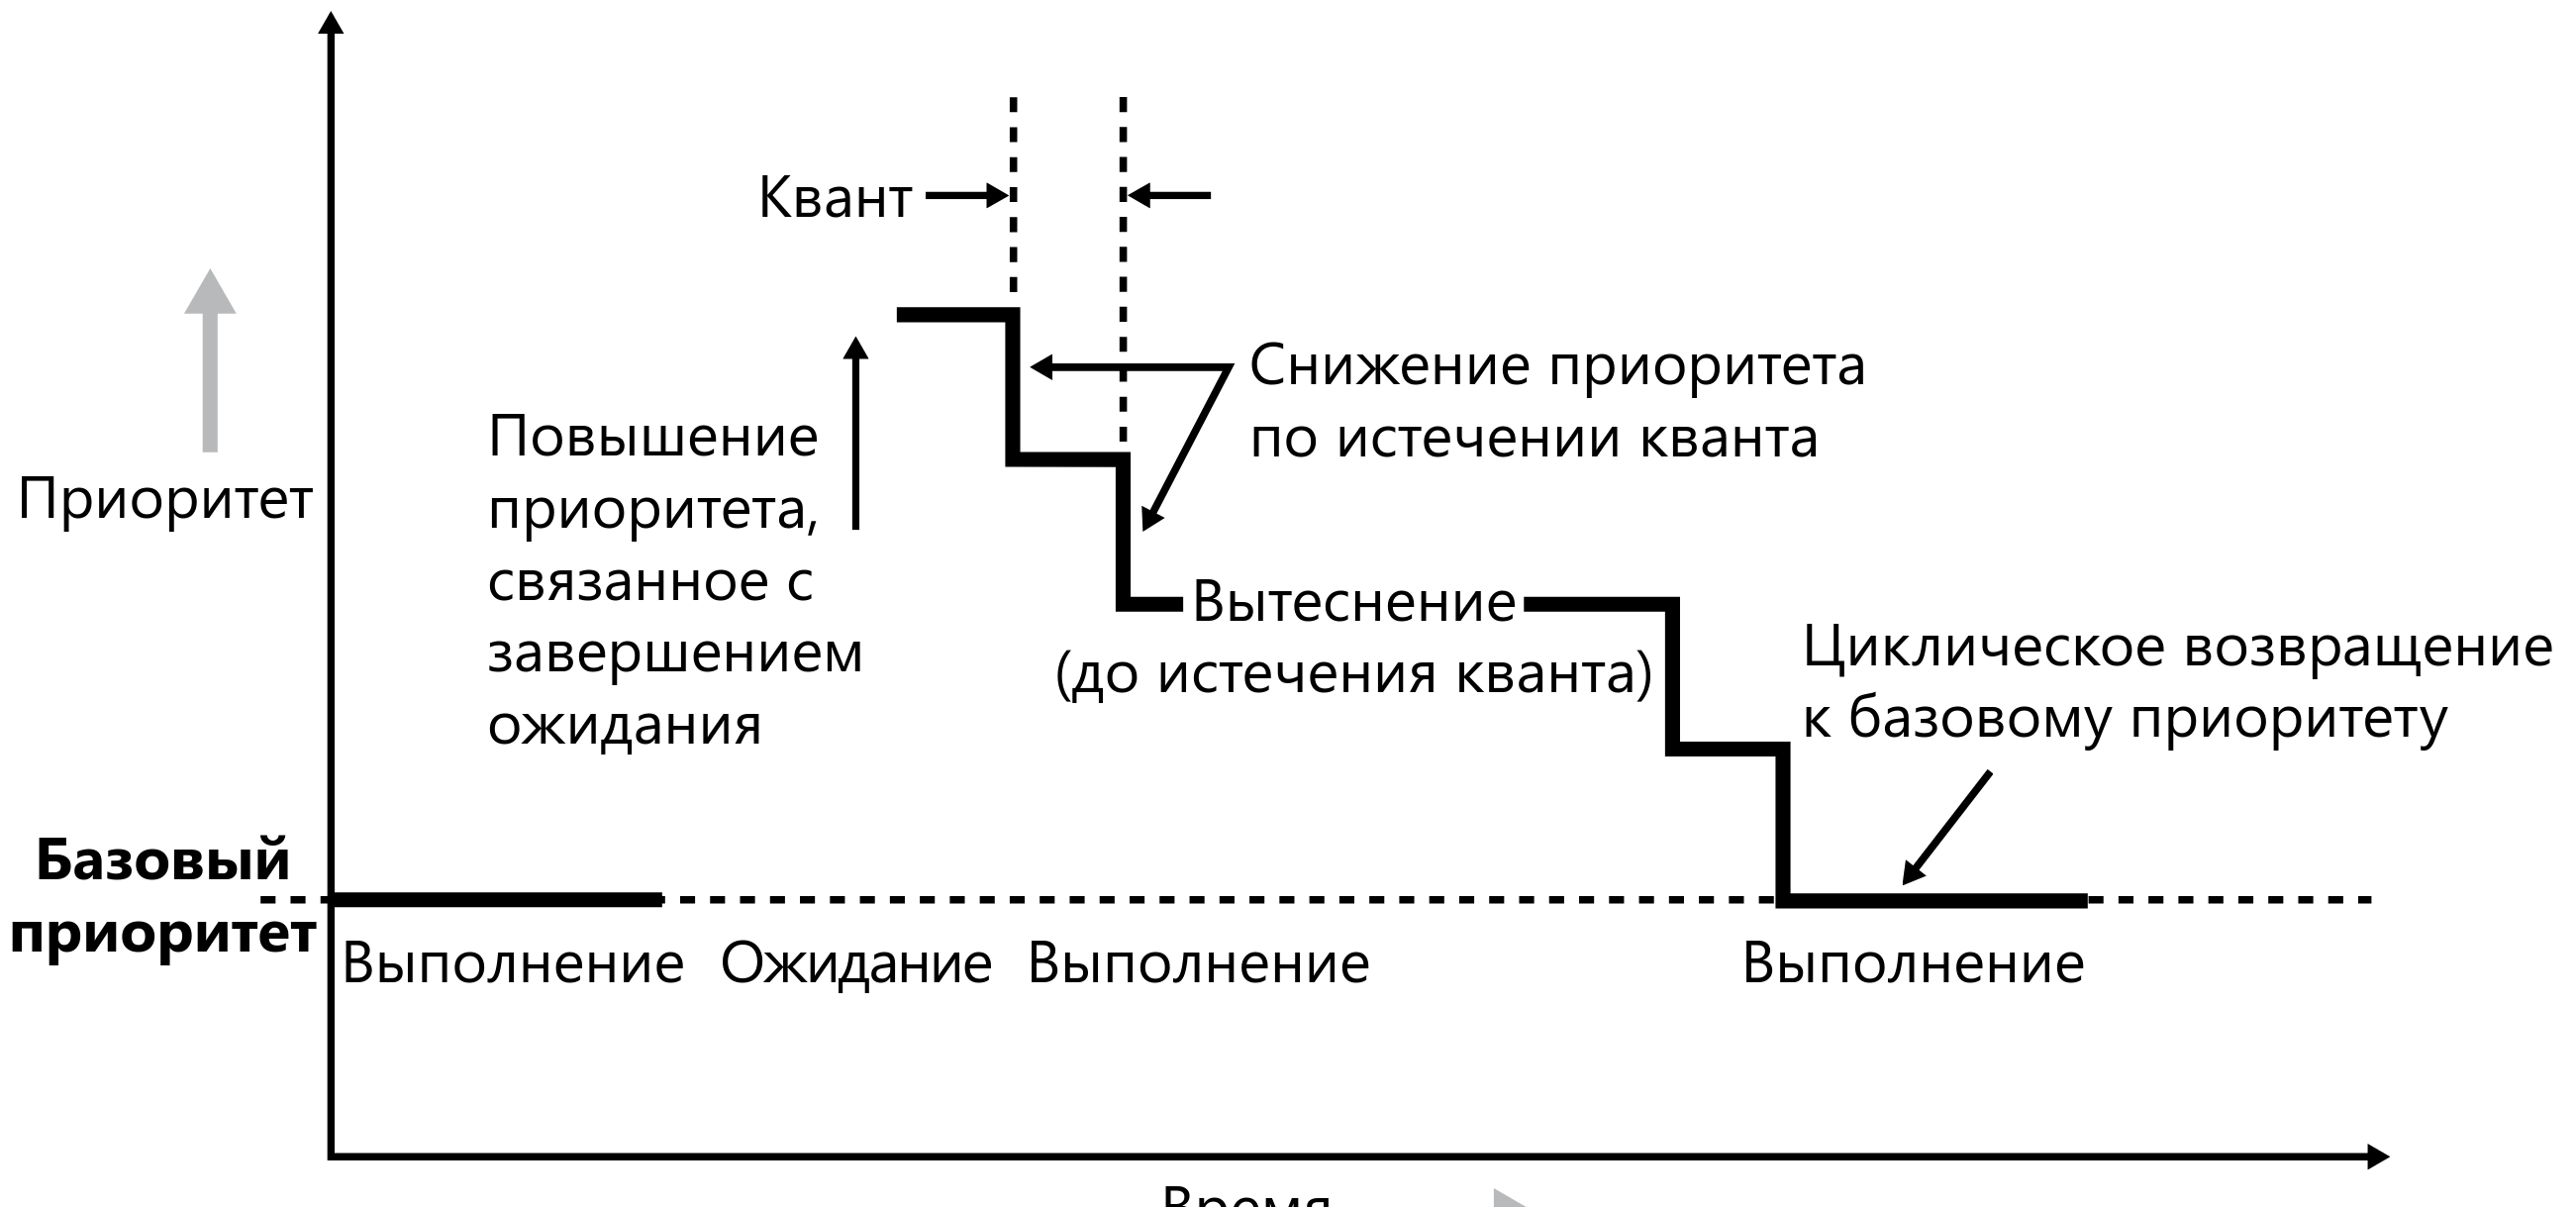
\includegraphics[width=0.6\textwidth]{priorgraph}
	\caption{Повышение и снижение приоритета}
	\label{fig:priorgraph}
\end{figure}

Для различных мультимедийных приложений, вроде воспроизведение видео/аудио, трёхмерных компьютерных игр требуются минимальные задержки, которые стандартные средства планировщика реализовать не могут, для клиентских версий была разработана служба MMCSS, чьей целью было гарантировать проигрывание мультимедийного контента приложений, зарегистрированных с этой службой, без каких-либо сбоев.

В действительности эта служба не повышает приоритет, как это делает планировщик, а меняет базовый приоритет процессов и потоков на время её работы. Важным свойством службы являются категории планирования, которые делят зарегистрированные процессы по приоритетам (представлены на рисунке~\ref{fig:mmcss}).

\begin{figure}[H]
	\centering
	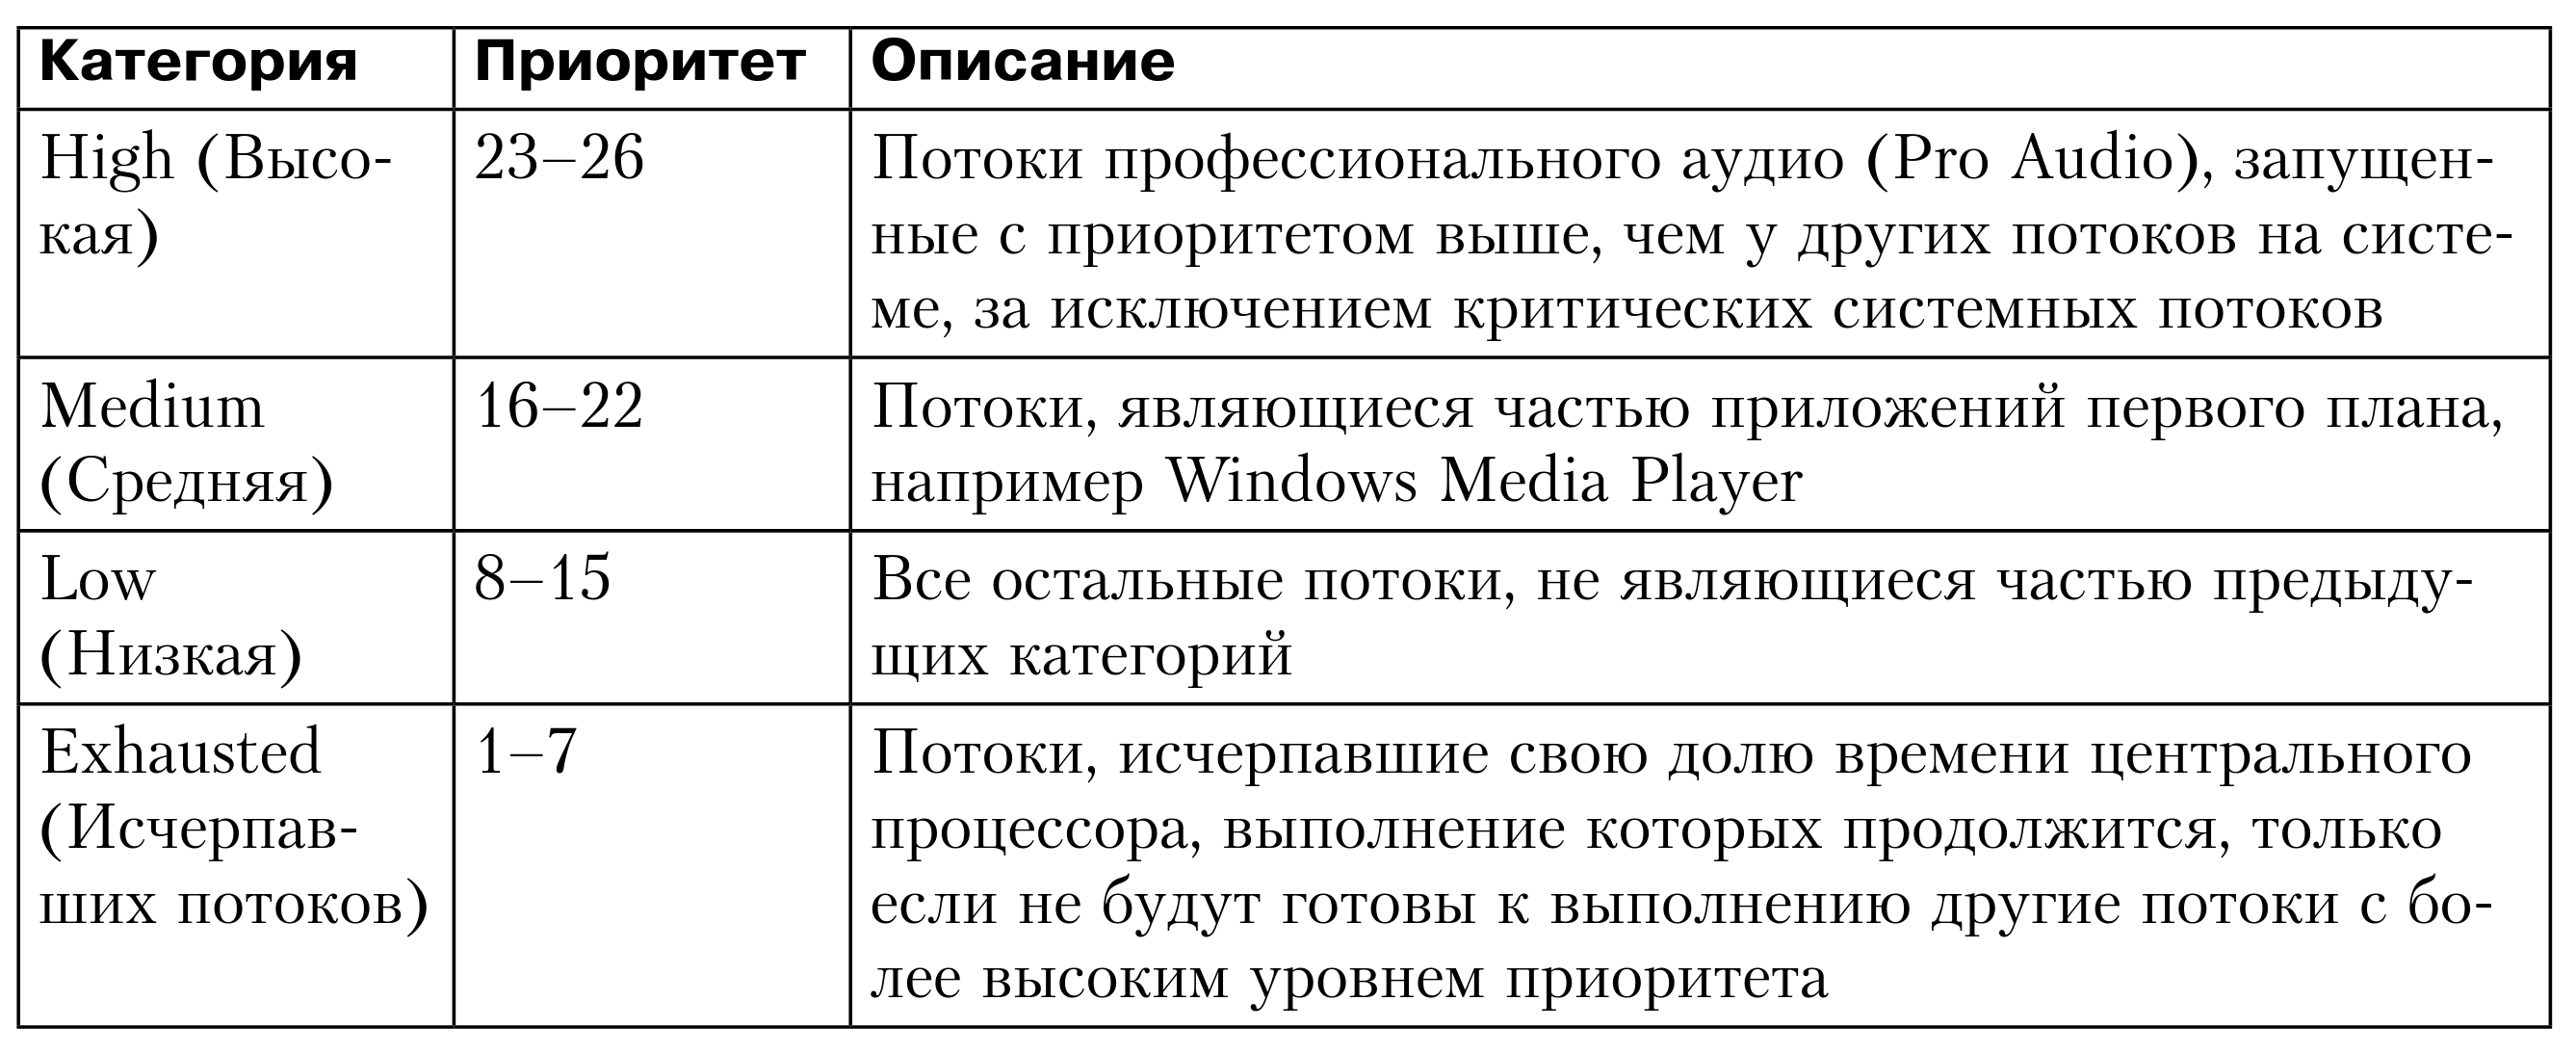
\includegraphics[width=0.9\textwidth]{mmcss}
	\caption{Категории планирования}
	\label{fig:mmcss}
\end{figure}

Механизм, положенный в основу MMCSS, повышает приоритет потоков внутри зарегистрированного процесса до уровня, соответствующего их категории планирования и относительного приоритета внутри этой категории на
гарантированный срок. Затем он снижает категорию этих потоков до Exhausted, чтобы другие, не относящиеся к мультимедийным приложениям потоки, также получили шанс на выполнение. По умолчанию мультимедийные потоки получают 80\% процессорного времени. При этом сама служба MMCSS выполняется с приоритетом 27, так как ей нужно вытеснить любые управляемые ей потоки.

\textbf{IRQL}

Контроллеры прерываний сами устанавливают приоритетность своих прерываний, однако Windows определяет свою схему приоритетности, называемую IRQL, которая представлена на рисунке~\ref{fig:IRQL}.

\begin{figure}[H]
	\centering
	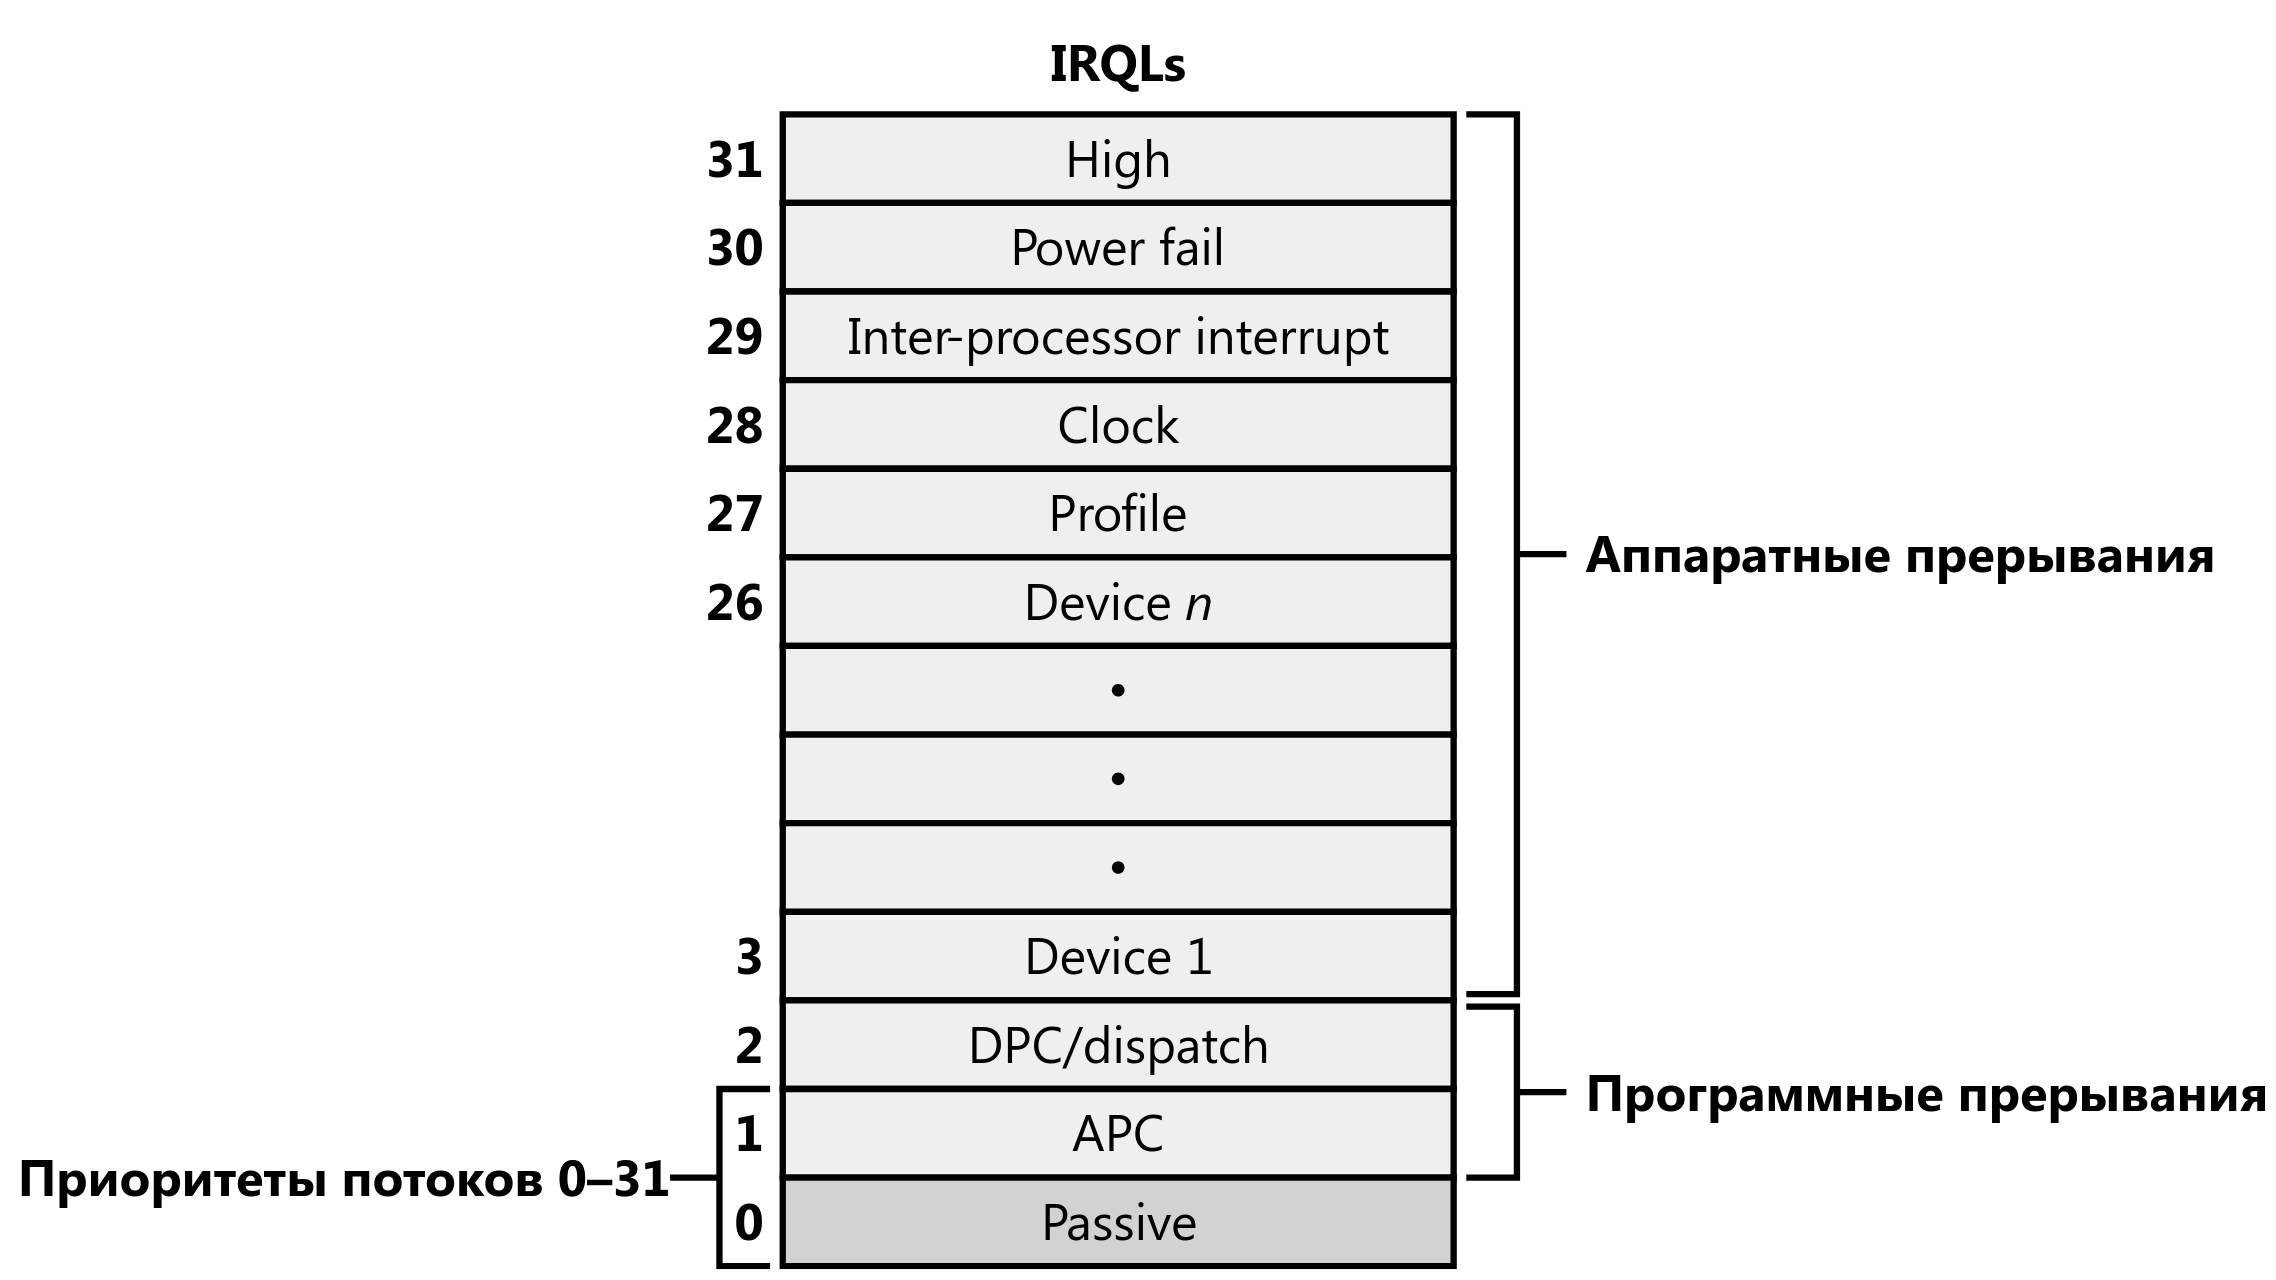
\includegraphics[width=0.6\textwidth]{IRQL}
	\caption{Сопоставление приоритетов потоков с IRQL-уровнями на системе x86}
	\label{fig:IRQL}
\end{figure}

Потоки обычно запускаются на уровне IRQL 0 или на уровне IRQL 1 (APC-уровень). Код пользовательского режима всегда запускается на пассивном уровне. Поэтому никакие потоки пользовательского уровня независимо от их приоритета не могут даже заблокировать аппаратные прерывания.

Потоки, запущенные в режиме ядра, несмотря на изначальное планирование на пассивном уровне или уровне APC, могут поднять IRQL на более высокие уровни, например, при выполнении системного вызова, который может включать в себя диспетчеризацию потока, диспетчеризацию памяти или ввод-вывод. Если поток поднимает IRQL на уровень dispatch или еще выше, на его процессоре не будет больше происходить ничего, относящегося к планированию потоков, пока уровень IRQL не будет опущен ниже уровня dispatch, так как прерывания обрабатываются в порядке из приоритетности. Поток выполняется на dispatch-уровне и выше, блокирует активность планировщика потоков и мешает контекстному переключению на своем процессоре.


\clearpage

\ssr{ЗАКЛЮЧЕНИЕ}

Так как семейства операционных систем Windows и Unix являются системами разделения времени, то функции их обработчиков системного таймера схожи. Основные из них:

\begin{itemize}
	\item Декремент кванта, по окончанию которого инициализируется диспетчеризация, которая передаёт квант другому процессу;
	\item Инкремент счётчиков времени;
	\item Инициализация работы планировщика;
	\item Декремент счётчиков отложенных вызовов.
\end{itemize}

В обоих семействах также используются динамически пересчитываемые приоритеты, которые решают позволяют работу нескольких процессов и решают проблемы бесконечного откладывания.

\ssr{СПИСОК ИСПОЛЬЗОВАННЫХ МАТЕРИАЛОВ}

\begin{enumerate}
	\item Вахалия Ю. UNIX изнутри. - СПб.: Питер, 2003. - 844 с.
	\item Робачевский А. Операционная система UNIX. - СПб.: БХВ-Петербург, 2002. - 528 с.
	\item Руссинович М., Соломон Д. Внутреннее устройство Microsoft Windows. - 6-e изд. - СПб.: Питер, 2013. - 800 с.
\end{enumerate}
